%%%%% Projekt z předmětu IMP %%%% 
%% Autor: Dominik Vágner, xvagne10

\documentclass[a4paper, 12pt]{article}
\usepackage[utf8]{inputenc}
\usepackage[T1]{fontenc}
\usepackage[czech]{babel}
\usepackage[text={18cm,25cm}, top=1.8cm, left=1.8cm, includefoot]{geometry}
\usepackage{graphicx}
\usepackage{amsmath}
\usepackage{float}
\usepackage{pdflscape}
\usepackage{cite}
\usepackage{etoolbox}
\usepackage{hyperref}
\usepackage{enumitem}

\patchcmd{\thebibliography}{\section*{\refname}}{}{}{}

\nocite{*}

\newcommand{\logo}{
    
\includegraphics[scale=0.1,keepaspectratio]{fig/logo_cz.png}
}

\title{\logo \\ \vspace{1.5em} IMP -- Projekt, varianta č. 21 \\ ESP32: Měření srdečního tepu [digitální senzor] \vspace{1em}}
\author{Dominik Vágner, \\ xvagne10}
\date{\today}

\begin{document}
    \maketitle

    \tableofcontents

    \newpage

    % Úvod %
    \section{Úvod}
Zadáním projektu bylo implementovat měřič srdečního tepu a míry okysličení krve pro mikrokontroler ESP32, pomocí digitálního senzoru z kterého měli tyto hodnoty být zobrazeny na OLED displeji.


    % Problematika %
    \section{Problematika}
Problematiku si můžeme do rozdělit do dvou částí a to inicializace sběrnic a komponentů, následná práce s nimi a zpracování z nich získaných dat.

\subsection{Inicializace sběrnic a komponentů}
Každá z našich externích komponent komunikuje s mikrokontrolerem pomocí jiné sběrnice. Náš OLED displej používá sběrnici SPI, zatímco náš senzor tepu komunikuje na sběrnici I2C. Jako první věc v našem programu, před hlavní smyčkou, musíme inicializovat naše komponenty a jejich sběrnice. Při inicializaci musíme specifikovat jaké jsou čísla GPIO pinů které používáme, jejich mód, povolení pull-up rezistorů a jejich frekvenci. Prvotní inicializace senzoru také vyžaduje nastavení jeho konfiguraci, kde nastavujeme jeho hodnoty určující například délku pulzu, nebo proud jednotlivých LED.



\subsection{Práce s komponenty a získanými daty}
S displejem naše práce vypadal velmi přímočaře. Jediné jsme potřebovali udělat bylo zvolit rozlišení, font a při zachycení srdečního pulzu smazat aktuálně zobrazený obsah displeje a nechat vykreslit nový s aktuálními hodnotami.

U senzoru už je situace komplikovanější, protože z něj přímo hodnoty které potřebujeme zobrazovat nedostáváme. Data které můžeme číst jsou pouze sečtené hodnoty střídavého a stejnosměrného proudu. Tyto data jsou také v senzoru ukládané do fronty z které je musíme číst a potvrzovat jejich přečtení pro posunutí fronty \cite{max30102-datasheet}. Z přečtených dat musíme nejdříve nejdříve odstranit hodnoty stejnosměrného proudu a následně musíme data vyfiltrovat a z výsledků rozhodnout zda jsme detekovali nový puls. Pokud byl puls detekován tak musíme vypočítat počet pulsů neboli tepů za minutu a kyslíkovou saturaci. 

Počet srdečních tepů za minutu počítáme tak že vydělíme délku minuty v milisekundách délkou jednotlivého pulsu, z těchto dat také děláme klouzavý průměr abychom dosáhli více srozumitelných výsledků. 

Kvadratický průměr potřebný pro výpočet kyslíkové saturace můžeme vypočítat pomocí rovnice \eqref{eq:R}, jedná se o vydělení střídavých a stejnosměrných proudů červené a infračervené diody. 
\begin{equation}\label{eq:R}
    R=\frac{\frac{A C_{\text {red }}}{D C_{\text {red }}}}{\frac{A C_{\text {infrared }}}{D C_{\text {infrared }}}}
\end{equation}
Po získaní daného průměru poté provedeme lineární aproximaci kyslíkové saturace. Po upravení hodnot z doporučených nastavení \cite{max30102-application-node} výrobci čipu tak aby seděl na testovaný kus (v porovnání s komerčním měřičem kyslíkové saturace a tepu, viz sekce \ref{testovani}) se došlo na rovnici \eqref{eq:SpO2}
\begin{equation}\label{eq:SpO2}
    SpO2 = 117 - 18R
\end{equation}

\newpage

    % Implementace %
    \section{Implementace}
Před počátkem implementace bylo třeba propojit mikrokontroler s komponenty umístěných na nepájivém poli.
\begin{figure}[h]
    \centering
    \medskip
    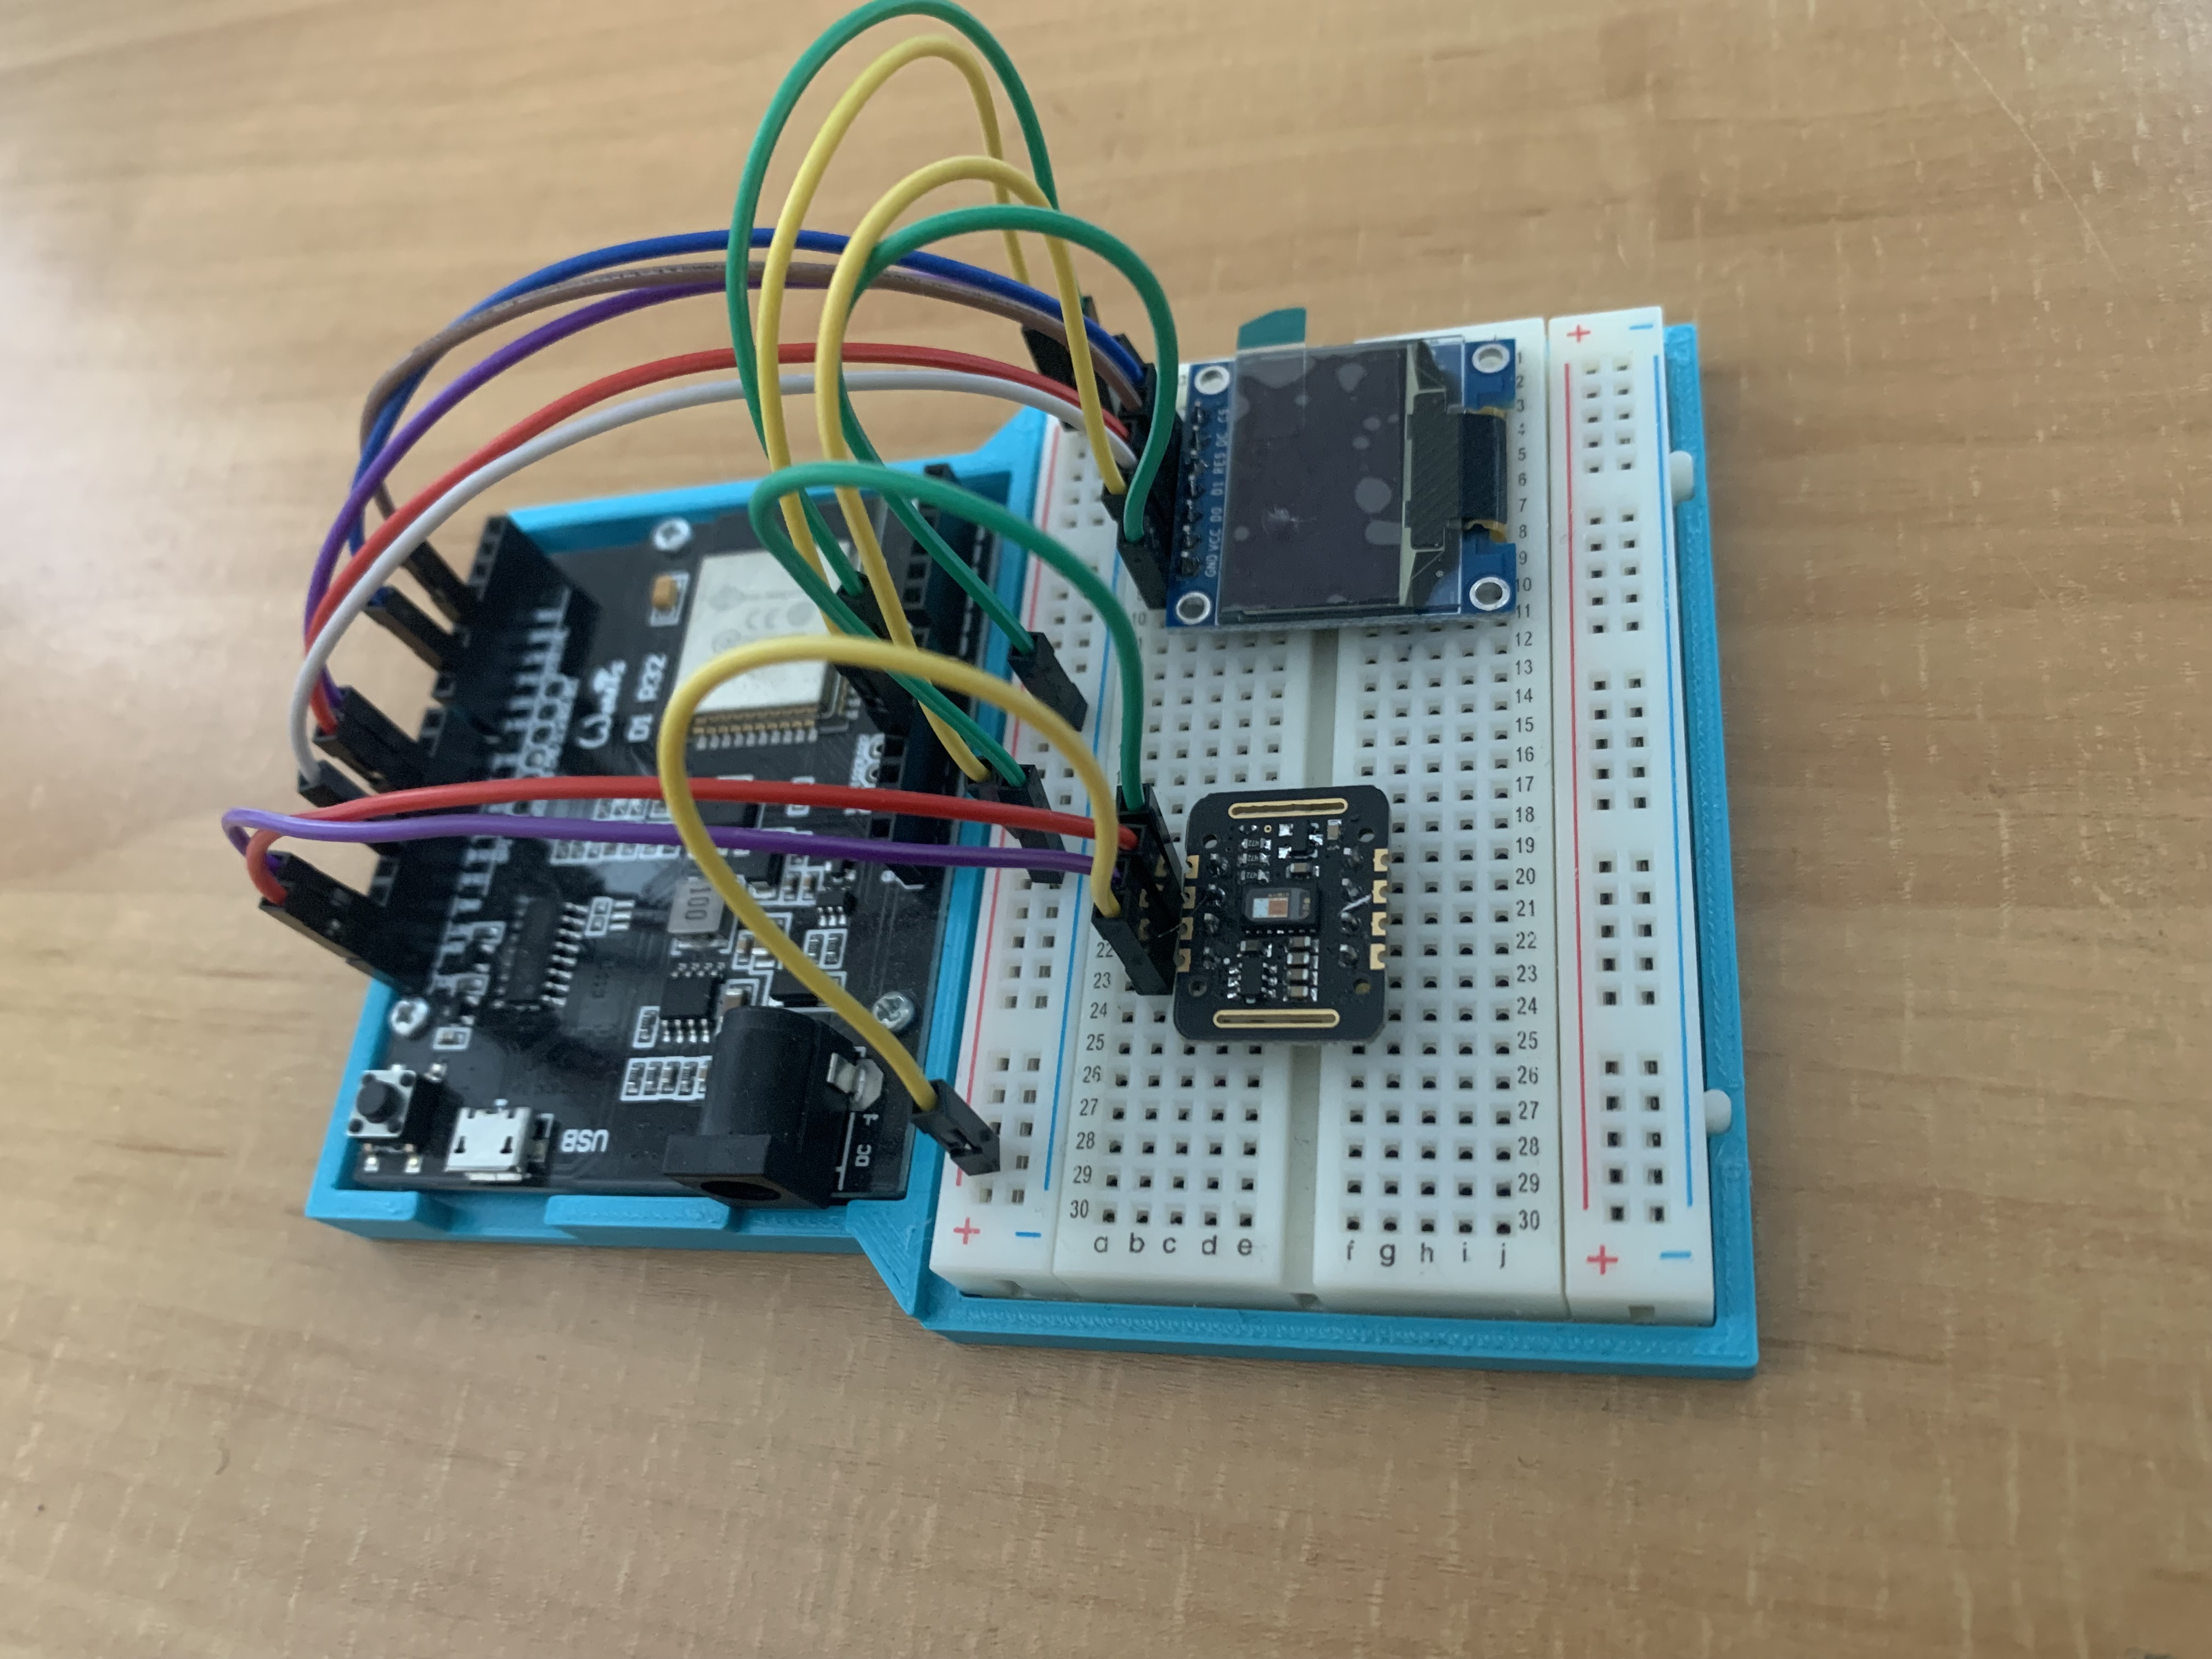
\includegraphics[scale=0.05]{fig/IMG_3925.jpeg}
    \medskip
    \caption{Zapojení komponent}
    \label{fig:obr1}
\end{figure}

Práci s displejem za nás řeší knihovna, která nám poskytuje font a příkazy pro vykreslení textu a mazání obsahu displeje \cite{ssd1306-lib}. Pro senzor máme taky většinu ze zmiňovaných problémů jako interakci s frontou, zpracování přerušení nebo výpočet počtu tepů za minutu nebo kyslíkové saturace za nás řeší s pomocí knihovny \cite{max30102-eps-idf-lib}. U této knihovny bylo potřeba pro lepší výsledky udělat menší úpravy a nastavení jiných hodnot než byly uvedené v ukázkách.

\subsection{Funkce}
\begin{itemize}[itemsep=0pt]
    \item \texttt{sensor\_task} -- Nejdůležitější funkce programu která periodicky kontroluje zda se vyskytl srdeční puls a případně obnoví hodnoty zobrazené na displeji novými nově získanými ze senzoru.
    \item \texttt{display\_init} -- Inicializuje displej za pomocí knihovny použité k jeho ovládání.
    \item \texttt{sensor\_i2c\_init} -- Inicializování I2C sběrnice pro senzor tepu.
    \item \texttt{sensor\_init} -- Inicializace a konfigurace senzoru tepu.
\end{itemize}

\subsection{Rozběhnutí projektu}
Projekt byl vytvářen s pomocí rozšířeni PlatformIO pro vývojové prostředí Visual Studio Code.
Po vytvoření projektu pro platformu Espressif ESP32 s použitým frameworkem ESP-IDF. Musíme do projektu vložit zdrojové kódy z odevzdaného archivu a nechat projekt přeložit a nahrát do mikrokontroleru. \\ \\
Poté po přiložení prstu na senzor tepu a míry oksyličení krve, by se na displeji měli automaticky začít vykreslovat hodnoty.

\newpage
    % Rozšíření %
    \section{Rozšíření}
Pro rozšíření projektu mě napadlo udělat z ESP mikrokontroleru taky Wi-Fi access point a na něm zprovoznit web server na kterém by se pravidelně obnovovali hodnoty, tedy stejně jako na displeji. Toto rozšíření mi přijde velmi praktické, chtěl jsem si ho vyzkoušet, protože by jej šlo využít i pro domácí prostředí kdybychom měli nějaký senzor a hodnoty z něho bychom chtěli mít přístupné odkudkoliv. Také by poté šlo vynechat zobrazování na displeji a zjednodušila by se tak komplexita zapojení a snížila se tak i cena.

\subsection{Funkce potřebné pro rozšíření}
\begin{itemize}[itemsep=0pt]
    \item \texttt{wifi\_init} -- Inicializace a konfigurace ESP jako Wi-Fi přístupového bodu \cite{setup-esp-as-AP}.
    \item \texttt{http\_init} -- Inicializuje HTTP server a přidání dvou koncových bodů \cite{http-server-setup}. 
    \item \texttt{index\_handler} -- Vytvoření obsluhy pro koncový bod \texttt{/}, který zobrazuje stejné hodnoty jako displej a pomocí asynchronních dotazů na koncový bod \texttt{/values} je obnovuje.
    \item \texttt{values\_handler} -- Vytvoření obsluhy pro koncový bod \texttt{/values}
\end{itemize}

    % Testovaní %
    \section{Testování} \label{testovani}
Projekt byl testován oproti komerčnímu produktu pro měření tepu a krevní kyslíkové saturace. Hodnoty kyslíkové saturace se podařilo odladit až na téměř identické, ale u hodnot tepů za minutu se občas stane, že na chvíli vyskočí na moc vysoké hodnoty a pak se po chvilce vrátí zpět. Nepodařilo se úplně přesně zjistit příčinu tohoto jevu, ale nejpravděpodobněji se bude jednat o nedostatečné omezení okolního světla nebo nekonzistentní tlak na prstu na senzor. Také nejde vyloučit možnost chyby v knihovně. \\ \\
Výsledek a ukázku testování si lze prohlédnout zde \href{https://youtube.com/shorts/q-xtbRGM5ro?feature=share}{zde}.
    % Závěr %
    \section{Závěr}
Projekt považuji za zajímavý prvotní úvod do programování vestavěných systémů. Zároveň bylo zajímavé nakouknout do knihoven pro ovládání externích komponent.

\subsection*{Autoevaluace}
Na projektu si myslím, že se mi podařilo implementovat vše s plnou funkčností a to s kvalitně napsaným kódem. Také jsem projekt rozšířil i další funkcionalitu jako HTTP server. Myslím že zdokumentování by možná mohlo být kvalitnější, ačkoliv nevidím v něm zase natolik velké nedostatky. Projekt bych si tedy ohodnotil plným počtem.

    
    \newpage
    \section*{Literatura}

\bibliographystyle{czechiso}

\bibliography{literatura}

    \addcontentsline{toc}{section}{Literatura}
\end{document}